\chapter{The morphological dependence of quenching}\label{chap:morph}

\emph{The work in the following chapter has been published in \citet{smethurst15}.}


By studying the galaxies which have just left the `star forming sequence' (SFS; see left panel of Figure \ref{sfr_mass_col}), the nature of the quenching mechanisms which cause this departure can be probed. By investigating the \emph{degree} of quenching that has occurred in the blue cloud, green valley and red sequence and by comparing that amount across the three populations, we can apply constraints to the many possible quenching mechanisms outlined in Chapter \ref{chap:intro}. 

I have been motivated by a recent result suggesting that there are two contrasting evolutionary pathways through the green valley for different morphological types (\citealt{schawinski14}, hereafter S14). S14 used the exponentially declining star formation model, described in Section~\ref{qmod}, to obtain predicted optical and NUV colours for four possible SFHs through the green valley; two with fast quenching rates ($\tau = [0.001, 0.25]$ $\rm{Gyr}$) and two with slower quenching rates ($\tau = [1, 2.5]$ $\rm{Gyr}$) beginning at $t_q = 9~\rm{Gyr}$. These predicted optical and NUV colours were then compared to the observed colours of early- and late-type green valley galaxy colours. S14 then concluded that late-type galaxies quench with a slower rate and form a nearly static disc population in the green valley, whereas early-type galaxies quench with very rapid rates, transitioning through the green valley and onto the red sequence in $\sim 1$~Gyr \citep{Wong12}. 

Although this result showing morphologically dependent quenching is intriguing, the work of S14 is hindered for the following reasons: (i) the incompleteness of the galaxy sample; only definitively early- ($p_s \geq 0.8$) and late-type ($p_s \leq 0.8$) galaxies were studied, whereas galaxies classified with intermediate morphology were excluded, and (ii) the lack of statistics to support the conclusions. Here I use the same toy SFH model but implement \starpy ~in order to statistically study the star formation histories of galaxies of all morphologies across the colour magnitude diagram.


\section{Defining the Green Valley}\label{defGV}

To define which of the $126, 316$ galaxies of the \textsc{gz2-galex} sample are in the green valley, I looked to previous definitions in the literature defining the separation between the red sequence and blue cloud. For example, \citet{Baldry04} traced this bimodality with a large sample of $66,846$ local SDSS galaxies ($0.004 < z < 0.08$) by fitting double-peaked Gaussians to the colour magnitude diagram. Their relation between the $u-r$ colour, $C'_{ur}$, and r-band magnitude, $M_r$, to define the colour cut between the blue and red galaxy populations is defined in their Equation 11 as:
\begin{equation}\label{eqgv}
C'_{ur}(M_{r}) = 2.06 - 0.244 \tanh \left( \frac{M_r + 20.07}{1.09}\right).
\end{equation}

Due to the necessity for NUV photometry in this study, matching to GALEX removed typical `red and dead' galaxies from the \textsc{gz2-galex} sample. This is apparent in the optical $u-r$ colour histograms shown in the right panels of Figure \ref{fig:cmgvsplit}; the \textsc{gz2-galex} sample is split in bins of absolute r-band magnitude and for each bin the position of the green valley at that $M_r$, as defined by \citet{Baldry04} is shown. For the \textsc{gz2-galex} sample at brighter r-band magnitudes (i.e. larger mass), this definition of the green valley seems to intersect with the observed peak at red colours. 

\begin{figure}
\centering{
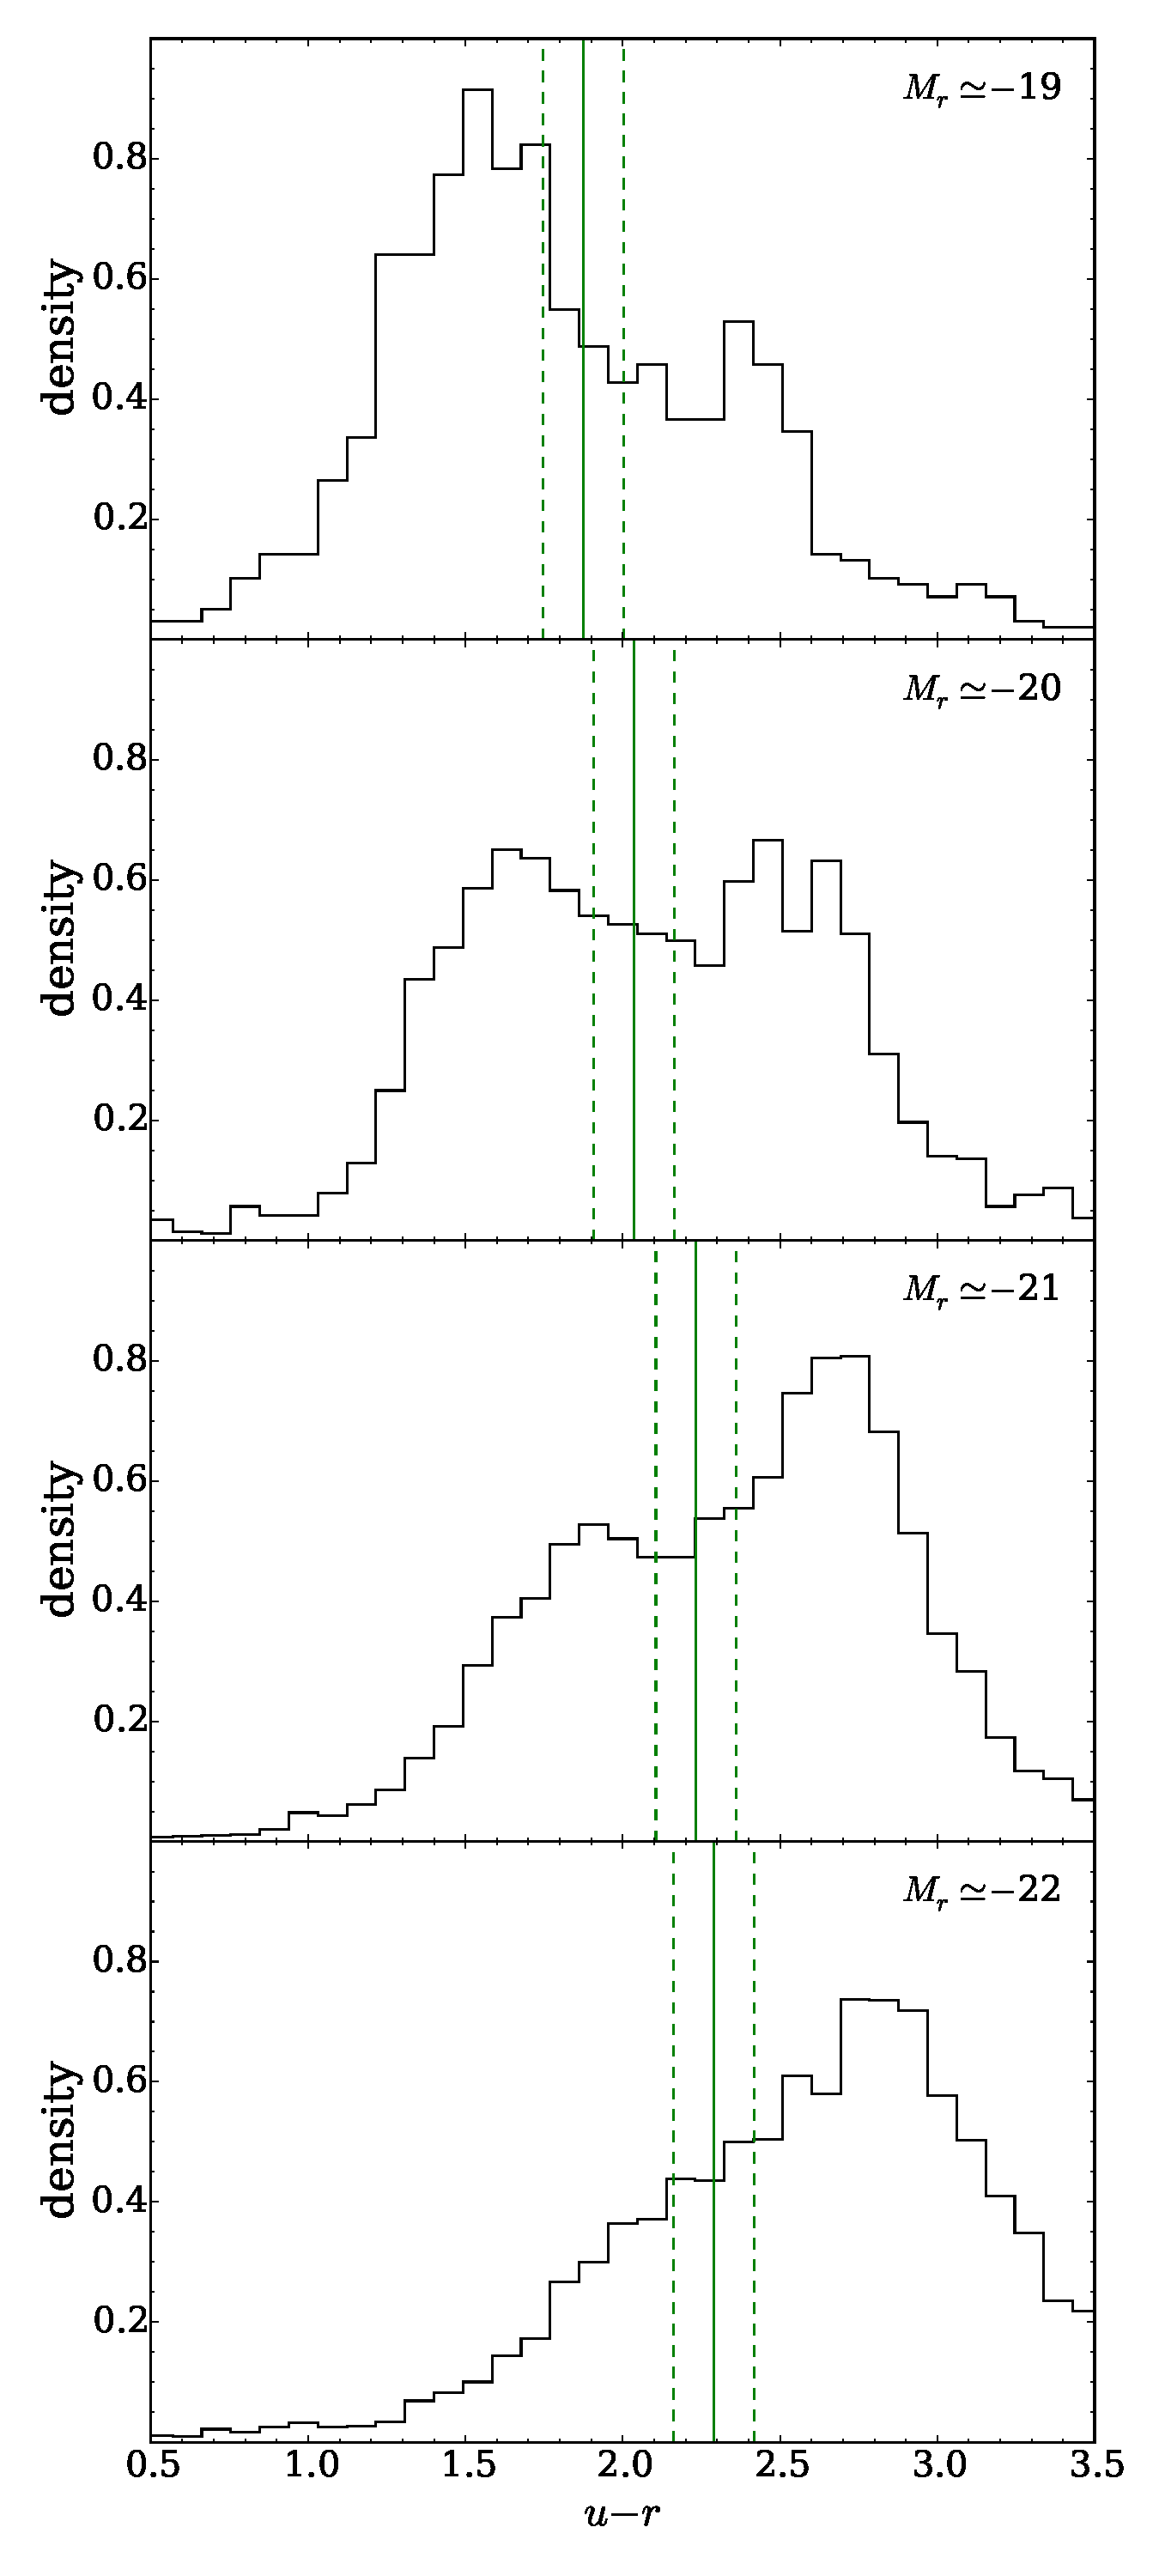
\includegraphics[width=0.49\textwidth]{morphology/sdss_hist_slice.pdf}
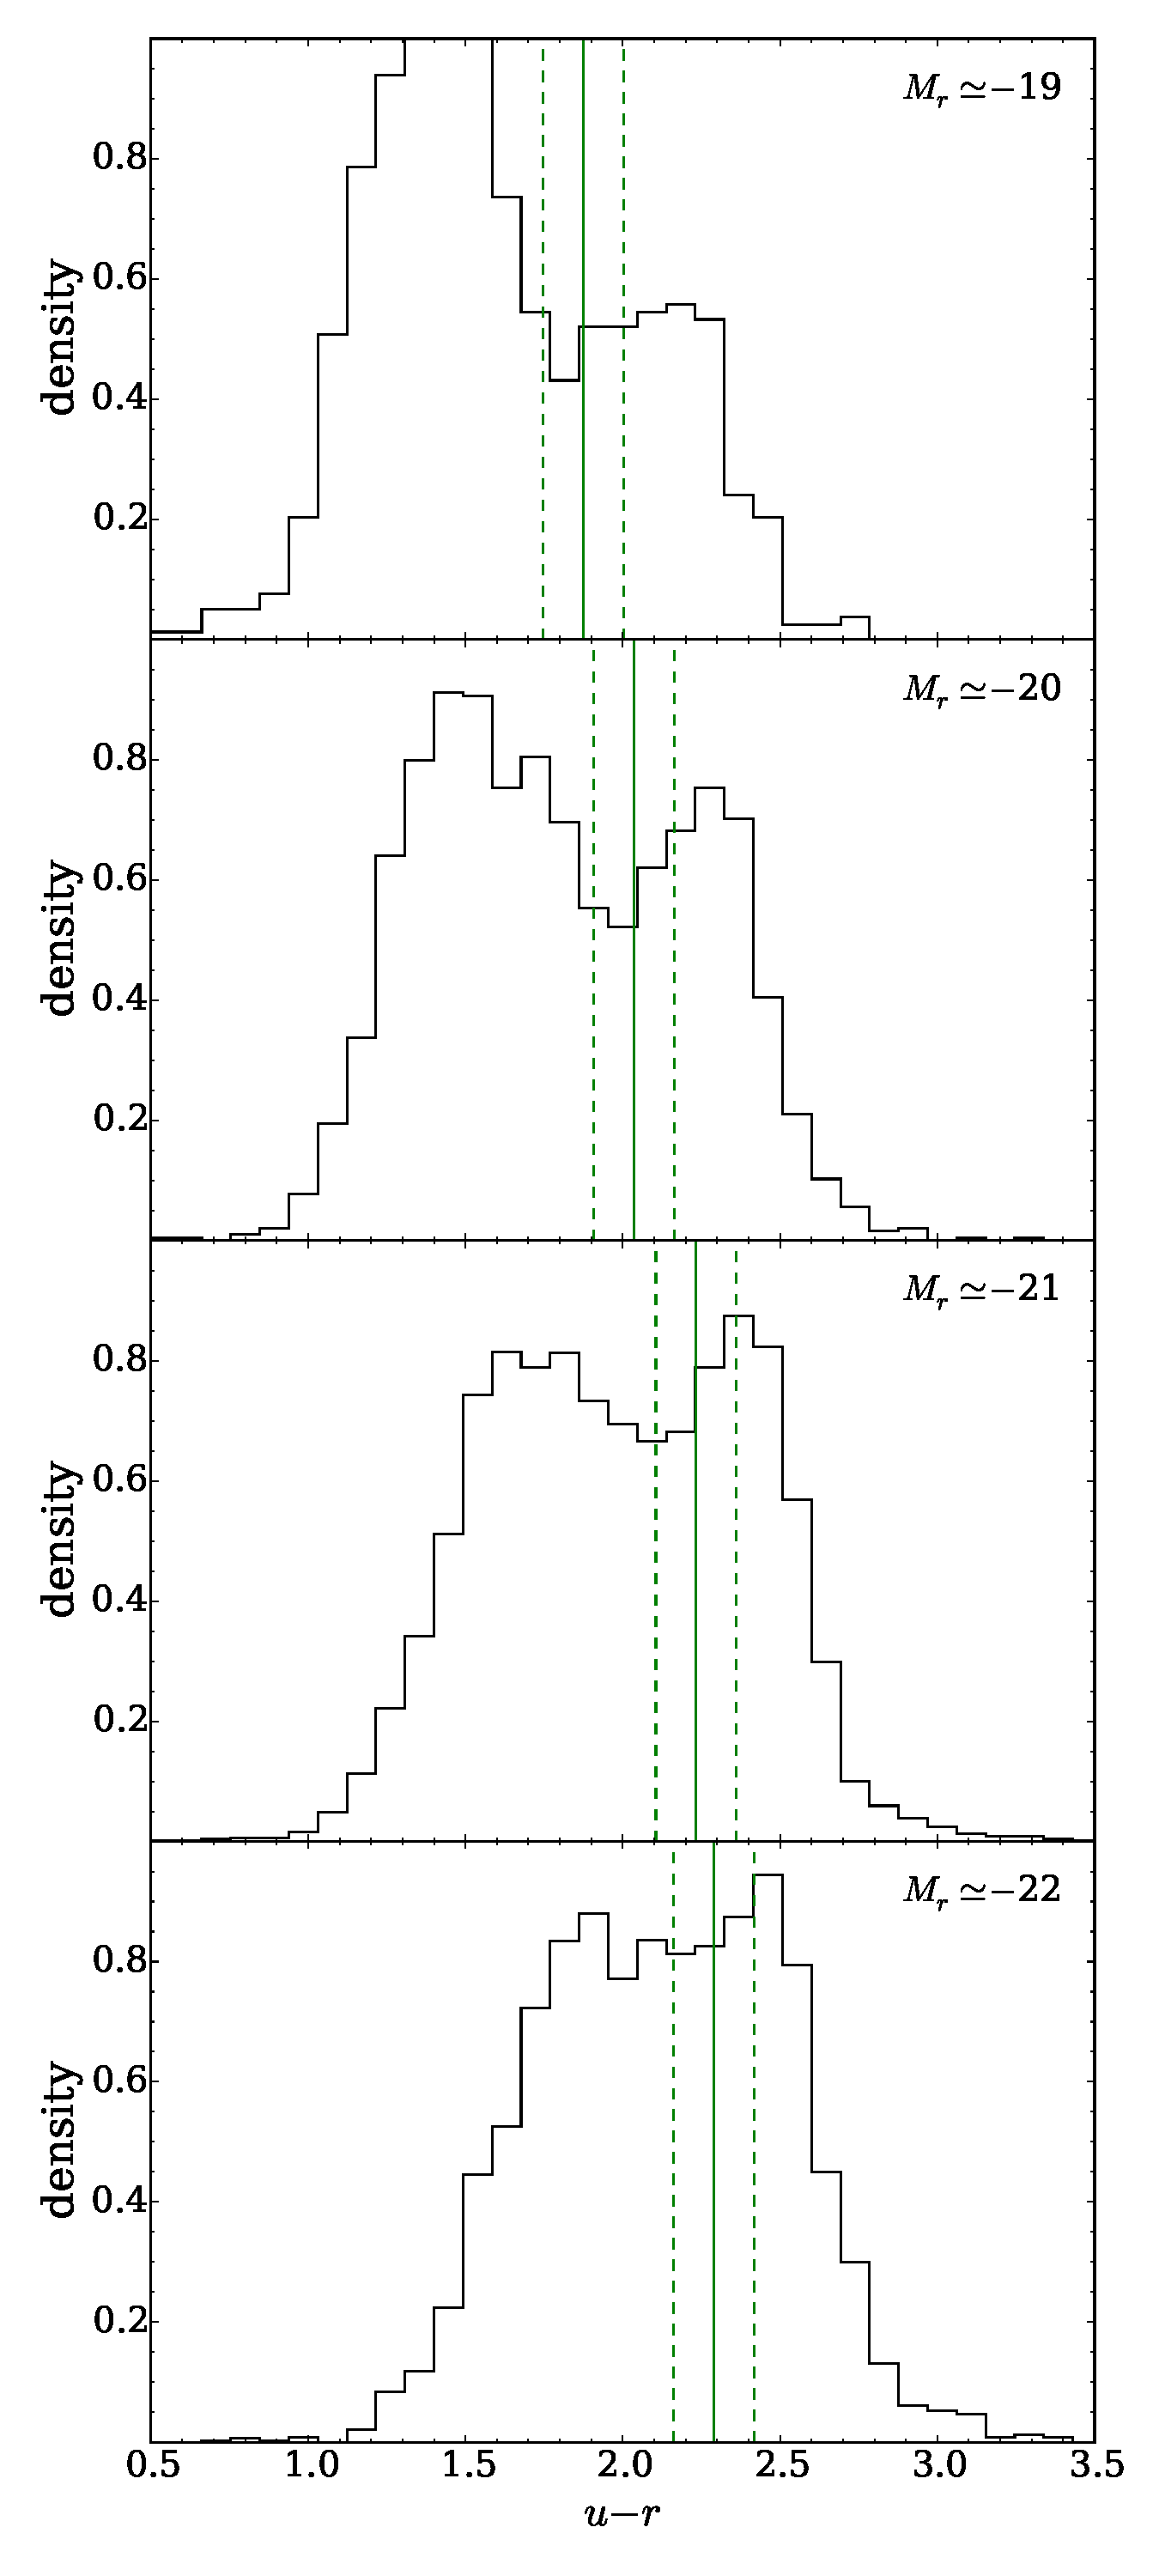
\includegraphics[width=0.49\textwidth]{morphology/galzoo_hist_slice.pdf}}
\caption[Optical $u-r$ colour histograms in absolute r-band magnitude slices of the \textsc{gz2-galex} and Baldry et al. (2004) complete SDSS samples]{Optical $u-r$ colour histograms, sliced in absolute r-band magnitude for a complete SDSS sample (MPA-JHU catalog; left) and for the \textsc{gz2-galex} sample (right). In each panel the definition between the blue cloud and the red sequence from \citet{Baldry04} is shown by the dashed line (as defined in Equation~\ref{eqgv}); the solid lines show $\pm 1\sigma$ either side of this definition.}
\label{fig:cmgvsplit}
\end{figure}

However, for a more complete SDSS sample (from the MPA-JHU catalog; \citealt[][left panels of Figure~\ref{fig:cmgvsplit}]{kauffmann03, brinchmann04}) the \citet{Baldry04} green valley definition does not intersect with the peak at red colours, as this sample is complete, containing the high mass typical `red and dead' galaxies of the red sequence. It would therefore not be appropriate to define the green valley by a visual fit to the colour magnitude diagram for this sample (this method was used in S14 and adopting it here would have allowed for a direct comparison to this previous work) as this would cause green valley galaxies to be misclassified as red sequence.

\begin{figure*}
\centering{
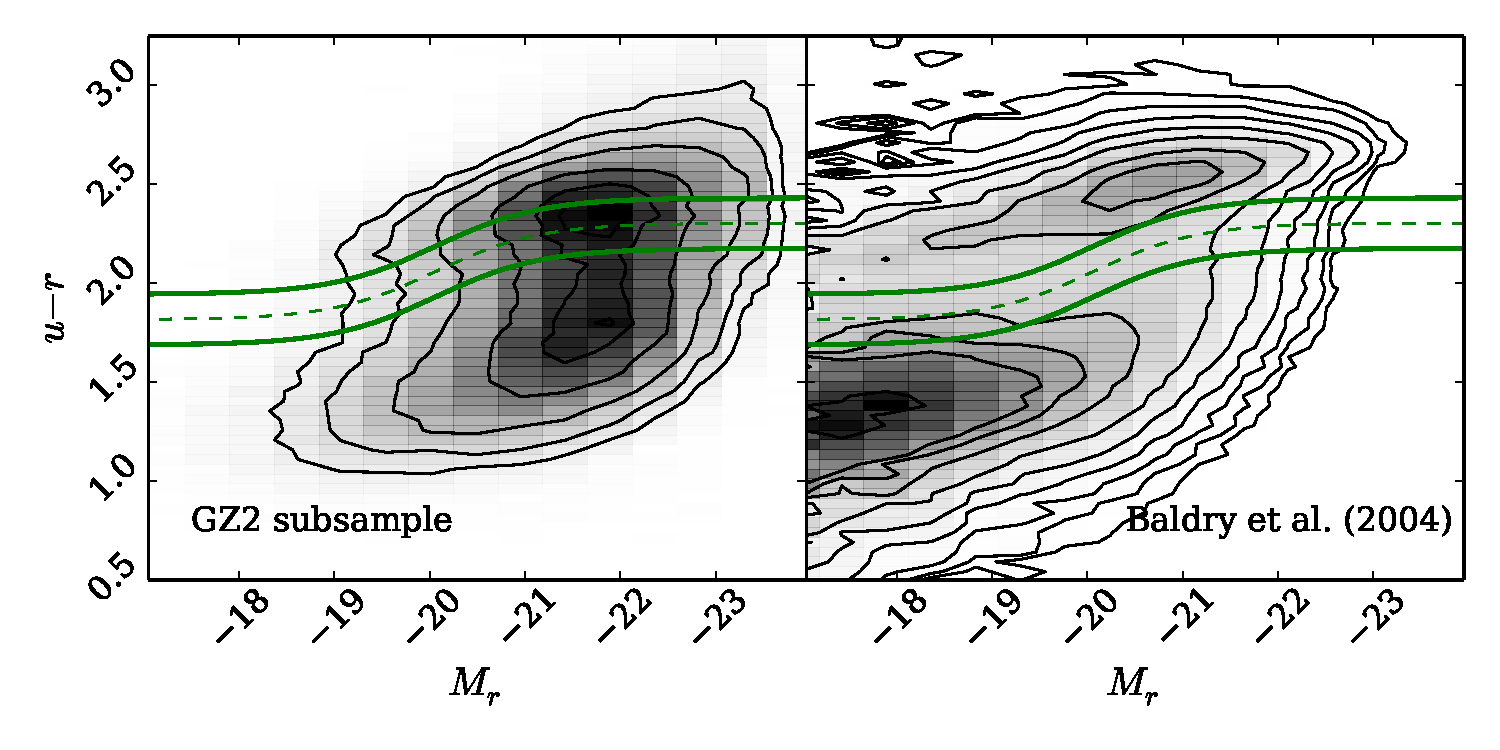
\includegraphics[width=\textwidth]{morphology/col_mag_GV_Baldry_data.pdf}}
\caption[Colour-magnitude diagram showing the location of the Baldry et al. (2004) green valley definition]{Colour-magnitude diagram for the \textsc{gz2-galex} sample (left) and the SDSS sample from \citet[][right]{Baldry04}. In both panels the definition between the blue cloud and the red sequence from \citet{Baldry04} is shown by the dashed line, as defined in Equation~\ref{eqgv}. The solid lines show $\pm 1\sigma$ either side of this definition; any galaxy within the boundary of these two solid lines is considered a green valley galaxy. The lack of red sequence galaxies due to the necessity for NUV GALEX colours skews the apparent location of the green valley in the \textsc{gz2-galex} sample, therefore a literature definition of the green valley is used to ensure galaxies are correctly classified.}
\label{fig:CMGV}
\end{figure*}

I therefore adopt the \citet{Baldry04} green valley definition for this study, which is shown in Figure~\ref{fig:CMGV} by the dashed line, overlaid on both the \textsc{gz2-galex} sample (left) and the SDSS data used by \citet[][right]{Baldry04}. I employ a conservative definition of the green valley; any galaxy within $\pm 1\sigma$ of the \citeauthor{Baldry04} relationship, shown by the solid lines in Figure~\ref{fig:CMGV}, is therefore considered a green valley galaxy. 

Despite the requirement for NUV photometry, the \textsc{gz2-galex} sample still contains typical galaxies from across the entirety of the colour magnitude diagram, including the red sequence. \cite{ko13} show that in a sample of quiescent red-sequence galaxies without $\mathrm{H}\alpha$ emission (i.e. without optical spectral indication of recent star formation), $26\%$ show NUV excess emission and that the fraction with mid-IR indication of recent star formation is $39\%$. Therefore this requirement for NUV photometry still allows for the selection of typical red sequence galaxies. Using the definition of the star forming SFS from \citet[][see Section~\ref{qmod}]{peng10} I find that $94\%$ of the red sequence galaxies in the \textsc{gz2-galex} sample lie more than $1\sigma$ below the main sequence; see Table ~\ref{table:qsubs}). 

The decomposition of the \textsc{gz2-galex} sample into red sequence, green valley and blue cloud galaxies is shown in Tables~\ref{table:subs} and \ref{table:qsubs} along with further division by galaxy type and SFR (where available for the \textsc{gz2-galex} sample from the MPA-JHU catalog) respectively. The tables also list the definitions I adopt henceforth for early-type ($p_s~ \geq~0.8$), late-type ($p_d~ \geq~0.8$), smooth-like ($p_s~ >~0.5$), disc-like ($p_d~ >~0.5$), quenched ($\rm{SFR}$ $ < P - 5\sigma$), quenching ($P - 5\sigma < \rm{SFR}$ $< P - \sigma$) and star forming  ($\rm{SFR}$ $> P -\sigma$) galaxies, where $P$ is the SFR as defined by \citet{peng10} for a given stellar mass and observed time (see Equation \ref{eq:peng}). 

\begin{table}
\caption{Table showing the decomposition of the \textsc{gz2-galex} sample by galaxy type into the subsets of the colour-magnitude diagram.}
\begin{tabular*}{\textwidth}{l @{\extracolsep{\fill}}cccc}
\hline
\begin{tabular}[c]{@{}c@{}} {\color{white} -} \\ {\color{white} -}  \end{tabular} & All                                                      & Red Sequence                                              & Green Valley                                              & Blue Cloud \\  \hline 
Smooth-like ($p_s > 0.5$)        & \begin{tabular}[c]{@{}c@{}}42453\\ (33.6\%)\end{tabular} & \begin{tabular}[c]{@{}c@{}}17424\\ (61.9\%)\end{tabular}  & \begin{tabular}[c]{@{}c@{}}10687\\ (44.6\%)\end{tabular}   & \begin{tabular}[c]{@{}c@{}}14342\\ (19.3\%)\end{tabular}  \\ 
Disc-like ($p_d > 0.5$)          & \begin{tabular}[c]{@{}c@{}}83863\\ (80.7\%)\end{tabular} & \begin{tabular}[c]{@{}c@{}}10722\\ (38.1\%)\end{tabular}   & \begin{tabular}[c]{@{}c@{}}13257\\ (55.4\%)\end{tabular}  & \begin{tabular}[c]{@{}c@{}}59884\\ (47.4\%)\end{tabular}  \\
Early-type ($p_s \geq 0.8$) & \begin{tabular}[c]{@{}c@{}}10517\\ (8.3\%)\end{tabular}  & \begin{tabular}[c]{@{}c@{}}5337\\ (18.9\%)\end{tabular}    & \begin{tabular}[c]{@{}c@{}}2496\\ (10.4\%)\end{tabular}    & \begin{tabular}[c]{@{}c@{}}2684\\ (3.6\%)\end{tabular}    \\
Late-type ($p_s \geq 0.8$)  & \begin{tabular}[c]{@{}c@{}}51470\\ (40.9\%)\end{tabular} & \begin{tabular}[c]{@{}c@{}}4493\\ (15.9\%)\end{tabular}    & \begin{tabular}[c]{@{}c@{}}6817\\ (28.5\%)\end{tabular}    & \begin{tabular}[c]{@{}c@{}}40430\\ (54.4\%)\end{tabular}  \\ \hline
\textbf{Total}                       & \begin{tabular}[c]{@{}c@{}}\textbf{126316} \\ (100.0\%)\end{tabular}                                                & \begin{tabular}[c]{@{}c@{}}28146 \\ (22.3\%)\end{tabular} & \begin{tabular}[c]{@{}c@{}}23944 \\ (18.9\%)\end{tabular} & \begin{tabular}[c]{@{}c@{}}74226 \\ (58.7\%)\end{tabular} \\\hline
\end{tabular*}
\label{table:subs}
\end{table}


\begin{table}
\caption{Table showing the decomposition of the \textsc{gz2-galex} sample by their star formation rate in the subsets of the colour-magnitude diagram.}
\begin{tabular*}{\textwidth}{l @{\extracolsep{\fill}}cccc}
\hline
\begin{tabular}[c]{@{}c@{}} {\color{white} -} \\ {\color{white} -}  \end{tabular} 		& All                                                      						& Red Sequence                                              			& Green Valley                                             			 & Blue Cloud \\  \hline 
\begin{tabular}[l]{@{}l@{}}Quenched\\ ($\rm{SFR} < P - 5\sigma$) \end{tabular}	& \begin{tabular}[c]{@{}c@{}}24278\\ (19.7\%)\end{tabular} 			& \begin{tabular}[c]{@{}c@{}}17018\\ (60.9\%)\end{tabular}    & \begin{tabular}[c]{@{}c@{}}6440\\ (27.5\%)\end{tabular}    & \begin{tabular}[c]{@{}c@{}}820\\ (1.1\%)\end{tabular}  \\ 
\begin{tabular}[l]{@{}l@{}}Quenching\\ ($P - 5\sigma < \rm{SFR} < P - \sigma$) \end{tabular}	 & \begin{tabular}[c]{@{}c@{}}34743\\ (28.2\%)\end{tabular}			 & \begin{tabular}[c]{@{}c@{}}9277\\ (33.1\%)\end{tabular}    & \begin{tabular}[c]{@{}c@{}}12181\\ (51.9\%)\end{tabular}    & \begin{tabular}[c]{@{}c@{}}13285\\ (18.6\%)\end{tabular}  \\ 
\begin{tabular}[l]{@{}l@{}}Star Forming  \\ ($\rm{SFR} > P -\sigma$) \end{tabular} & \begin{tabular}[c]{@{}c@{}}63957\\ (52.0\%)\end{tabular} 			& \begin{tabular}[c]{@{}c@{}}1665 \\ (5.9\%)\end{tabular}    & \begin{tabular}[c]{@{}c@{}}4828\\ (20.6\%)\end{tabular}    & \begin{tabular}[c]{@{}c@{}}57464\\ (80.3\%)\end{tabular}  \\ \hline
\textbf{Total}                       		& \begin{tabular}[c]{@{}c@{}}\textbf{122,978} \\ (100.0\%)\end{tabular} & \begin{tabular}[c]{@{}c@{}}27960 \\ (22.7\%)\end{tabular} & \begin{tabular}[c]{@{}c@{}}23449 \\ (19.1\%)\end{tabular} & \begin{tabular}[c]{@{}c@{}}71569 \\ (58.2\%)\end{tabular} \\\hline
\end{tabular*}
\label{table:qsubs}
\end{table}

Figure~\ref{sfr_mass_sub} shows the SFR against the stellar mass for the \textsc{gz2-galex} sample (where available from the MPA-JHU catalog) split into blue cloud, green valley, red sequence, late- and early-type populations. This figure (see bottom row, middle panel) confirms that the green valley galaxies in the \textsc{gz2-galex} sample are indeed a population which have either left, or begun to leave, the star forming SFS. A relatively small fraction ($20.6\%$; see Table~\ref{table:qsubs}) are also classified as star forming galaxies, however the middle panel, bottom row of Figure~\ref{sfr_mass_sub} shows that these galaxies reside on the low SFR side of the SFS.

\begin{figure*}
\centering{
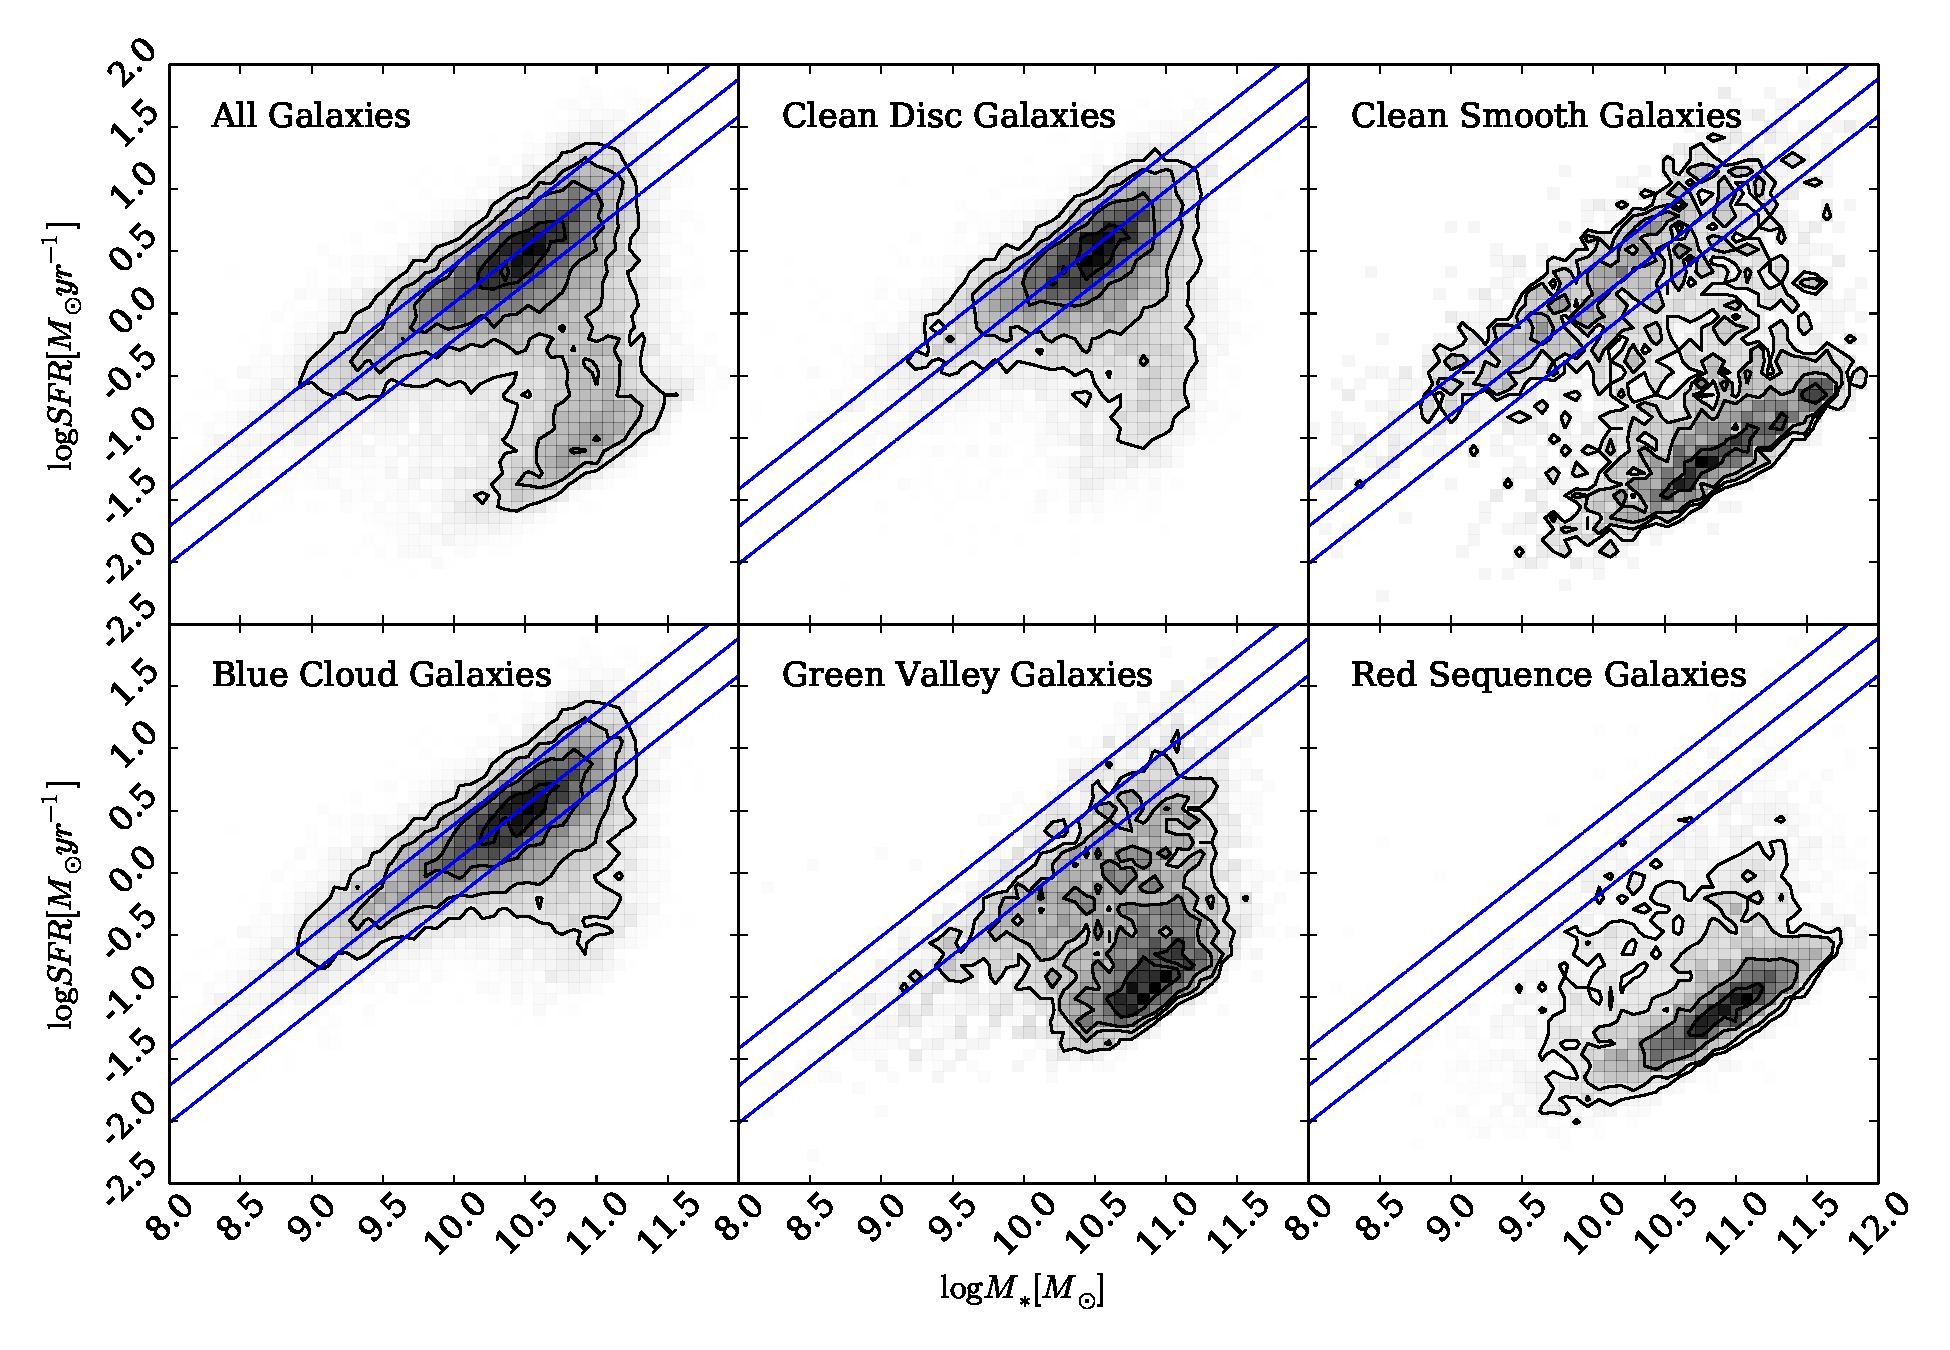
\includegraphics[width=\textwidth]{morphology/sfr_mass_subsets.pdf}}
\caption[SFR-stellar mass plane split by morphology and colour]{Star formation rate against stellar mass for the different populations of galaxies (top row, left to right: all galaxies, late-type galaxies, early-type galaxies; bottom row, left to right: blue cloud, green valley and red sequence galaxies) and how they contribute to the star forming sequence (from \citet{peng10}, shown by the solid blue line with 0.3 dex scatter by the dashed lines). Based on positions in these diagrams, the green valley does appear to be a transitional population between the blue cloud and the red sequence. Detailed analysis of star formation histories can elucidate the nature of the different populations' pathways through the green valley.}
\label{sfr_mass_sub}
\end{figure*}


\section{Results}\label{sec:morphresults}

The population density distributions for both smooth and disc weighted populations in the red sequence, green valley and blue cloud are shown in Figures~\ref{red_s},~\ref{green_v} \&~\ref{blue_c} respectively. The full two dimensional distributions in $[t, \tau]$ are shown in each case, along with a histogram showing the one dimensional projection for each individual parameter, marginalised over the other one. The percentages shown in Figures~\ref{red_s},~\ref{green_v} \&~\ref{blue_c} are calculated as the fractions of the population densities located in each region of parameter space for a given population. 

Since the sample contains such a large number of galaxies, a peak in the population densities will be caused by a large number of galaxies with peaks in their individual posterior distribution at that location in parameter space. This will overwhelm contributions to this area of the population density from galaxies where this region of parameter space is not dominant in their individual posterior distributions. Therefore these fractions can be interpreted as broadly equivalent to the percentage of galaxies in a given population undergoing quenching at a rate within the stated range. Although this is not quantitatively exact, it is nevertheless a useful framework for interpreting the population densities.

Figure~\ref{fig:bestfit} shows the distribution of the median walker positions (the 50th percentile of the posterior probability distribution) of each individual galaxy, split into red, green and blue disc-like ($p_d > 0.5$) and smooth-like ($p_s > 0.5$)  populations. This is done in order to incorporate the full \textsc{gz2-galex} sample and still investigate the morphological dependence of the results without discarding any data. Unlike in the \textsc{popstarpy} method (see Section \ref{popstarpy}) these plots were made without discarding any walker positions due to low probability and without weighting by the GZ2 morphological vote fractions. Figure~\ref{fig:bestfit} may therefore be more intuitive to understand than Figures~\ref{red_s},~\ref{green_v} \&~\ref{blue_c}.

Although the quenching rates are continuous in nature, in this Chapter I will refer to rapid, intermediate and slow quenching rates which correspond to ranges of  $\tau ~\rm{[Gyr]} < 1.0$, $1.0 < \tau ~\rm{[Gyr]} < 2.0$ and $\tau ~\rm{[Gyr]} > 2.0$ respectively for ease of discussion.



\subsection{The Red Sequence}\label{rs}

\begin{figure*}
\centering{
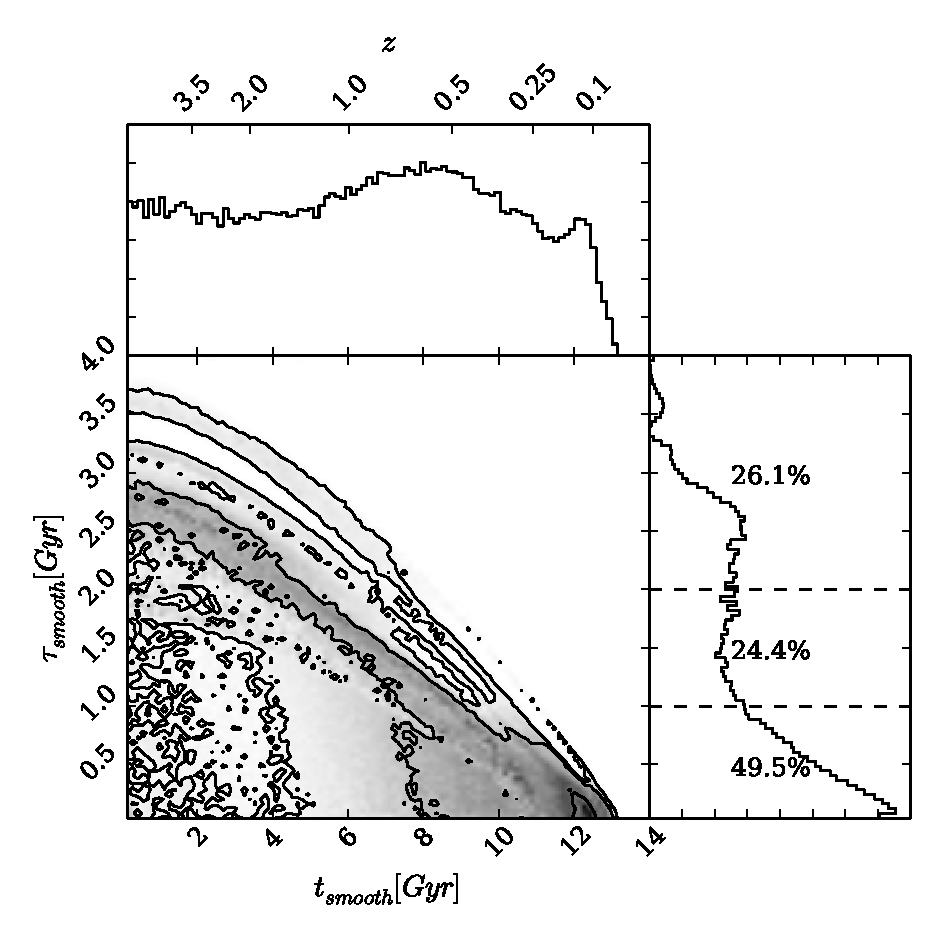
\includegraphics[width=0.55\textwidth]{morphology/red_smooth.pdf}\\
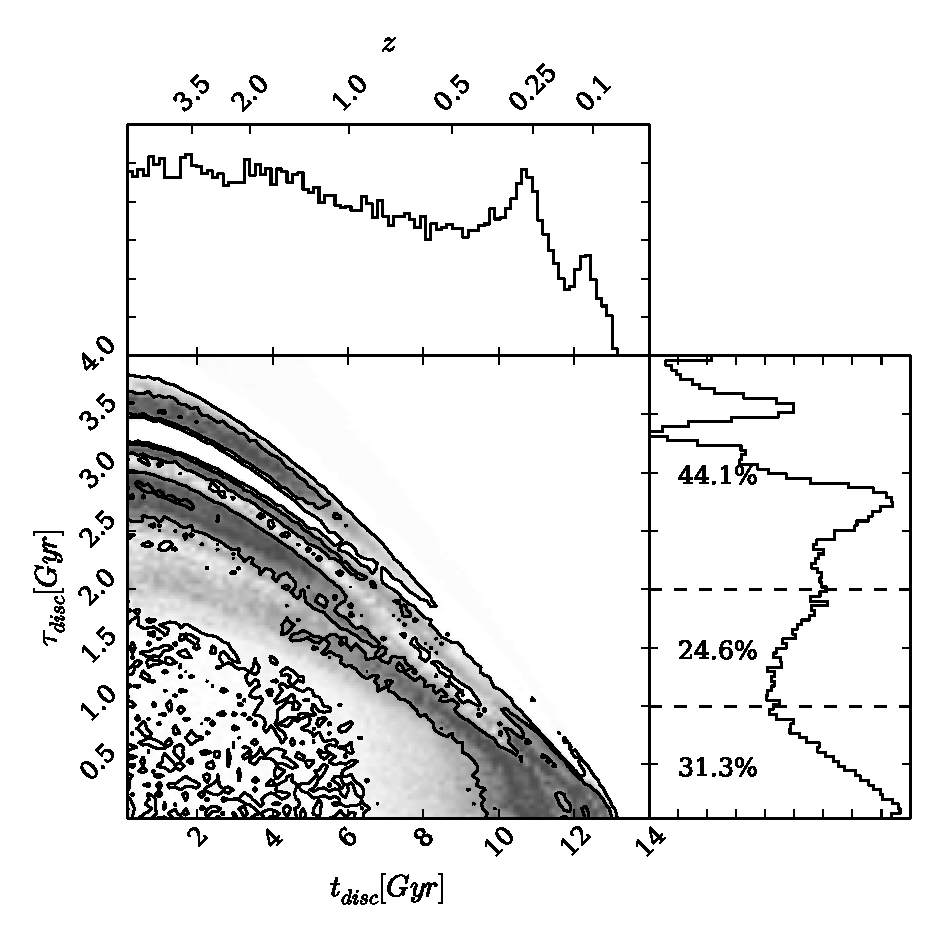
\includegraphics[width=0.55\textwidth]{morphology/red_disc.pdf}}
\caption[Smooth and disc weighted population densities of red sequence galaxies]{Contour plots showing the population densities for red sequence galaxies of the \textsc{gz2-galex} sample, weighted by the morphological vote fractions from GZ2 to give both bulge (top) and disc (bottom) dominated distributions. The histograms show the projection into one dimension for each parameter. The dashed lines show the separation between rapid ($\tau ~\rm{[Gyr]} < 1.0$), intermediate ($1.0 < \tau ~\rm{[Gyr]} < 2.0$) and slow ($\tau ~\rm{[Gyr]} > 2.0$) quenching rates with the fraction of the combined posterior probability distribution in each region shown (see Section~\ref{stats}).}
\label{red_s}
\end{figure*}

The top panel of Figure~\ref{red_s} reveals that the red sequence smooth weighted population density is dominated by rapid quenching rates (with an estimated $49.5\%$ of galaxies undergoing quenching at this rate; see Figure~\ref{red_s}). At early quenching times (high redshift) however, the population density is dominated by slow and intermediate rates (top panel of Figure~\ref{red_s}). Perhaps this is the influence of intermediate galaxies (with $p_s \sim p_d \sim 0.5$), which would explain why similar high density areas exist for both the smooth and disc weighted populations in both panels of Figure~\ref{red_s}. This is especially apparent considering there are far more of these intermediately classified galaxies than those that are definitively early- or late-types (see Table~\ref{table:subs}). 

The bottom panel of Figure~\ref{red_s} reveals a bimodal distribution for the disc weighted population density between rapid $(31.3\%)$ and slow $(44.1\%)$ quenching rates. The very slow ($\tau > 3.0 ~\rm{Gyr}$) quenching rates present in the red disc population density (which are not seen in either the green valley or blue cloud, see Figures~\ref{green_v} and~\ref{blue_c}) with $[t, \tau] \sim [1, 3.5]~\rm{Gyr}$ take approximately $11.5~\rm{Gyr}$ to transition to the red sequence in the SFH models. This suggests that these galaxies have only just reached the red sequence after a very slow evolution across the colour-magnitude diagram. Considering their limited number and the requirement for NUV emission, it is likely that these galaxies are currently on the edge of the red sequence having recently (and finally) moved out of the green valley. 

\citet{tojeiro13} used the VErsatile SPectral Analyses spectral fitting code (VESPA; \citealt{tojeiro07}) and found that red late-type spirals show 17 times more recent star formation than red elliptical galaxies. The results in Figure \ref{red_s} can be tested against this finding  by comparing the SFRs predicted by the inferred SFH model of both the smooth and disc weighted population densities (these SFRs are shown in Figure \ref{pred}). For the peak at early times and slow quenching rates in the red disc weighted population density, this SFH model still has some residual star formation occurring with a SFR$~\sim0.105~\rm{M}_{\odot}yr^{-1}$. Whereas for the peak at recent times and rapid quenching rates in the red smooth weighted population density, this SFH model has a resultant SFR$~\sim0.0075~\rm{M}_{\odot}yr^{-1}$. This is approximately 14 times less than the residual SFR still occurring in the red disc weighted population; within error, this is in agreement with the findings of \citet{tojeiro13}. 

These results for the red sequence galaxies have many implications for green valley galaxies, as all of these systems must have passed through the green valley on their way to the red sequence.


\subsection{Green Valley Galaxies}\label{gv}

\begin{figure*}
\centering{
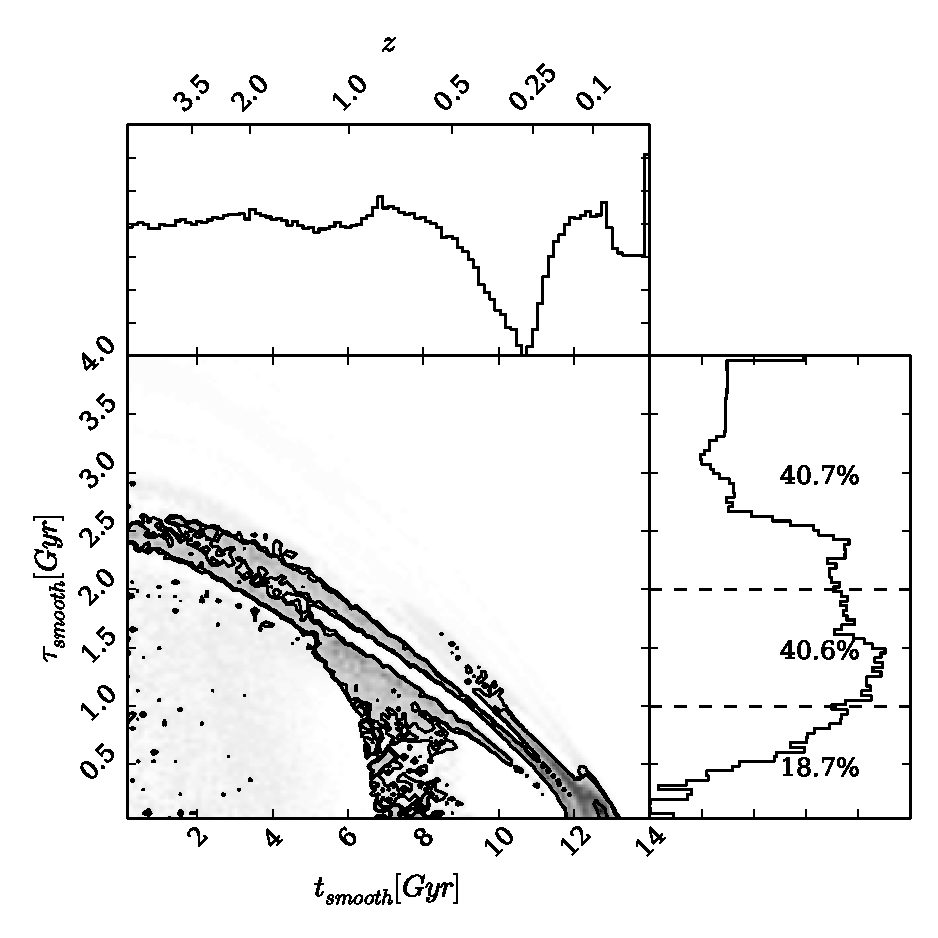
\includegraphics[width=0.55\textwidth]{morphology/green_smooth.pdf}\\
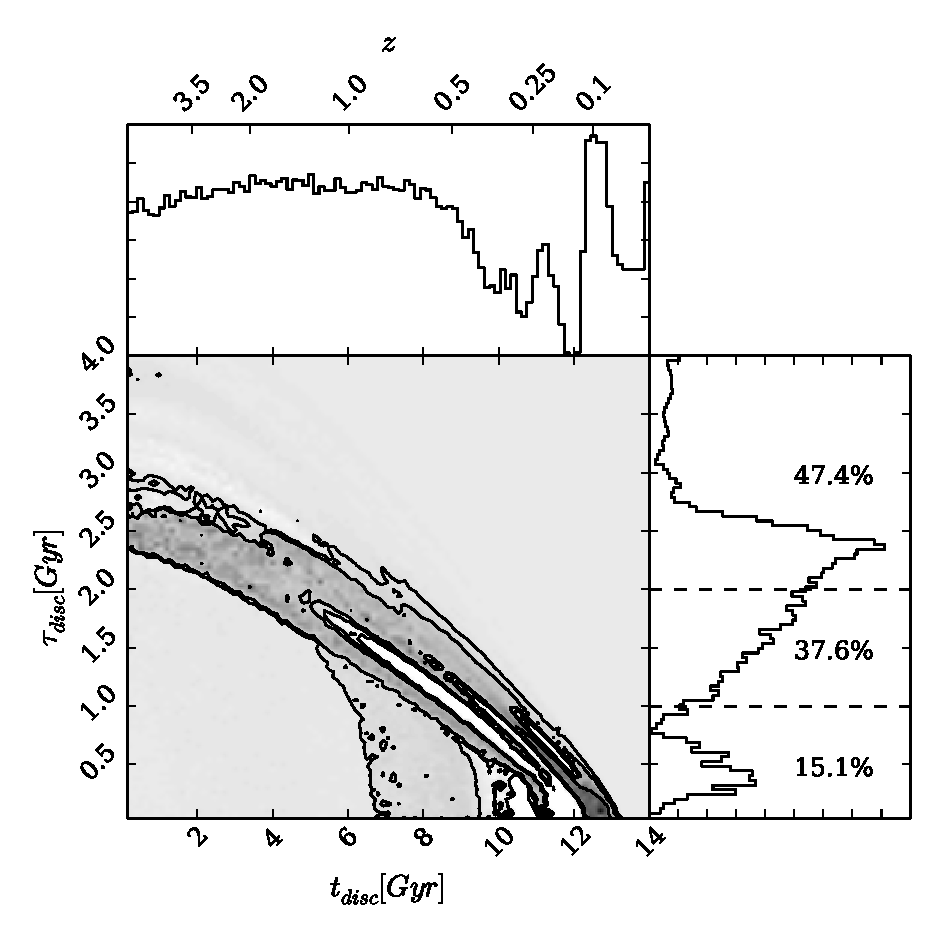
\includegraphics[width=0.55\textwidth]{morphology/green_disc.pdf}}
\caption[Smooth and disc weighted population densities of green valley galaxies]{Contour plots showing the population densities for green valley galaxies in the \textsc{gz2-galex} sample weighted by the morphological vote fractions from GZ2 to give both bulge (top) and disc (bottom) dominated distributions. The histograms show the projection into one dimension for each parameter. The dashed lines show the separation between rapid ($\tau ~\rm{[Gyr]} < 1.0$), intermediate ($1.0 < \tau ~\rm{[Gyr]} < 2.0$) and slow ($\tau ~\rm{[Gyr]} > 2.0$) quenching rates with the fraction of the combined posterior probability distribution in each region shown (see Section~\ref{stats}).}
\label{green_v}
\end{figure*}

Figure \ref{green_v} shows how the smooth weighted green valley population density is dominated by both intermediate quenching rates ($40.6\%$) and slow quenching at rates early times ($z > 1$; $40.7\%$). The fraction of the population density at rapid quenching rates in this smooth weighted population is half that seen in the red sequence smooth weighted population. This is caused, in part, by the fact that rapidly quenching galaxies will transition through the green valley very quickly. To quantify this I tested the time spent in the green valley across the $[t, \tau]$ parameter space assuming a stellar mass, $m = 10^{10.27} M_{\odot}$ (the mean mass of the \textsc{gz2-galex} sample), which is shown in Figure~\ref{fig:timeingv}. The galaxies with such a rapid decline in star formation rate spend very little time in the green valley, therefore fewer of these galaxies will reside in the green valley at any one time in comparison to those galaxies transitioning with slower quenching rates. However the amount of rapid quenching occurring across the entire galaxy population is not underestimated, as all galaxies which have undergone a rapid quenching history will now be found in the red sequence and detected there in the \textsc{gz2-galex} sample.  This contributes to the dominance of rapid quenching rates in the red sequence population densities (see Figure \ref{red_s}) and explains the observed number of intermediatly classified morphology galaxies (see Table \ref{table:subs}) which are present in the green valley (assuming a morphological change occurs during the quench).

\begin{figure*}
\centering{
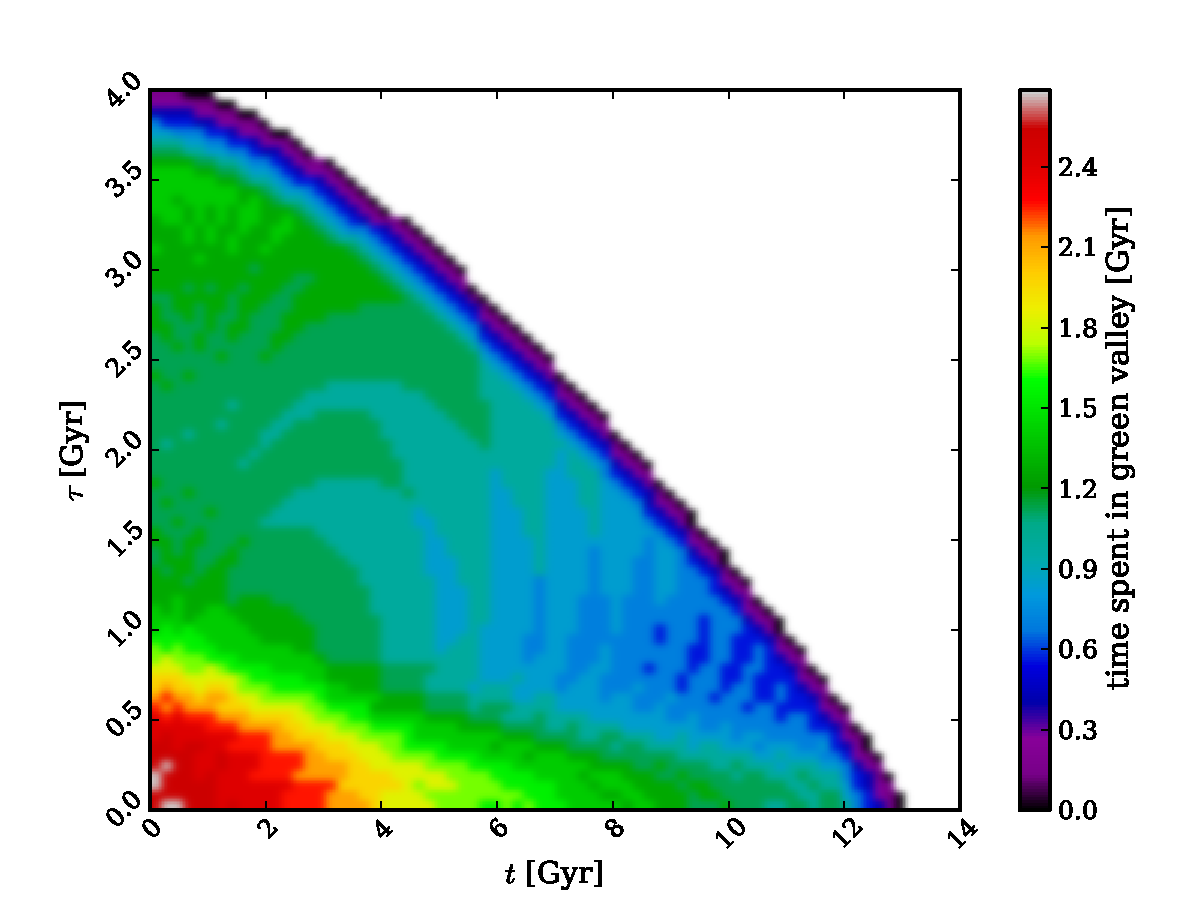
\includegraphics[width=0.9\textwidth]{morphology/green_valley_time.pdf}}
\caption[Time spent in the green valley across parameter space]{Plot showing the time spent in the green valley across the SFH model parameter space by the current epoch. This affects the observability of those galaxies which have quenched rapidly and recently and have passed too quickly through the green valley to be detected. The white region denotes those models with colours that do not enter the green valley by the present cosmic time.}
\label{fig:timeingv}
\end{figure*}

The green valley disc weighted population density is completely dominated by slow quenching rates ($47.4\%$) with a slightly smaller fraction of intermediate quenching rates detected than in the smooth weighted population ($37.6\%$; see Figure~\ref{green_v}).

If the population densities of Figures~\ref{green_v} \& \ref{red_s} are compared, quenching is detected at later cosmic times (lower redshift) in the green valley than in the red sequence for both morphological types. This therefore suggests that both morphologies are tracing the evolution of the red sequence (i.e. evolving with the same quenching histories just at a later time), confirming that the green valley is indeed a transitional population between blue cloud and red sequence regardless of morphology. 

Given enough time ($t\sim4 - 5~\rm{Gyr}$), the current green valley disc galaxies will therefore eventually transition through to the red sequence (the right panel of Figure~\ref{sfr_mass_col} shows galaxies with $\tau > 1.0~\rm{Gyr}$ do not approach the red sequence within $3~\rm{Gyr}$ post quench). This is most likely the origin of the `red spirals', attributed to the very slow quenching rates discussed in Section~\ref{rs} (and see bottom panel of Figure~\ref{red_s}). This is in contradiction to the conclusions of S14 who state that the disc population stall in the green valley. 

Considering this result that the green valley is a transitional population, the ratio of smooth~:~disc galaxies that is currently observed in the green valley is expected to evolve into the ratio observed in the red sequence (assuming that the decreased number of galaxies detected in the red sequence due to matching to GALEX is independent of morphology). Table~\ref{table:subs} shows the ratio of smooth-like~:~disc-like galaxies in the red sequence is $62:38$, whereas in the green valley this ratio is $45:55$. Making very simple assumptions that this ratio does not change with redshift and that quenching is the only mechanism which causes a morphological transformation, then $31.2\%$ of the disc-like galaxies in the green valley would have to undergo a morphological change to a smooth-like galaxy. 

Inspecting the disc weighted green valley population density (bottom panel of Figure~\ref{green_v}) reveals that $29.4\%$ of the distribution occupies the $\tau < 1.5 ~\rm{Gyr}$ parameter space. Since this is a similar fraction to the number of green valley disc-like galaxies which would have to undergo a morphological change to a smooth-like galaxy to match the ratio of smooth~:~disc galaxies in the red sequence, this suggests that quenching mechanisms with $\tau < 1.5 ~\rm{Gyr}$ are capable of destroying the disc-dominated structure of galaxies. 

All of this evidence suggests that there are not just two contrasting evolutionary pathways through the green valley for different morphological types as concluded by S14. The intermediate quenching rates reside in the space between the extremes sampled by the optical-NUV colour-colour diagrams of S14. The inclusion of the intermediately classified galaxies in this investigation and the use of a statistical method elucidates a continuum of quenching rates, with all galaxies transitioning through the green valley to the red sequence during quenching, regardless of morphology. 

Therefore instead of concluding that \emph{`the green valley is a red herring'} as in S14, I would conclude that the \emph{`grass is always redder on the other side'}.


\subsection{Blue Cloud Galaxies}\label{bc}

\begin{figure*}
\centering{
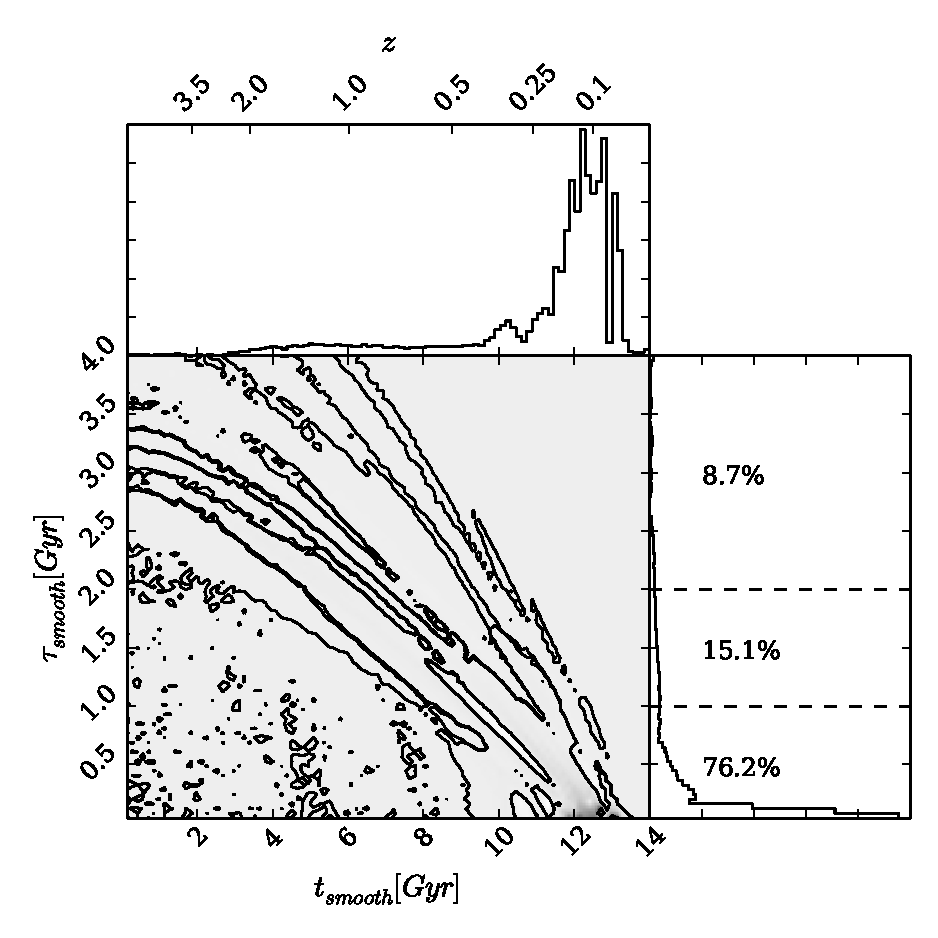
\includegraphics[width=0.55\textwidth]{morphology/blue_smooth.pdf}\\
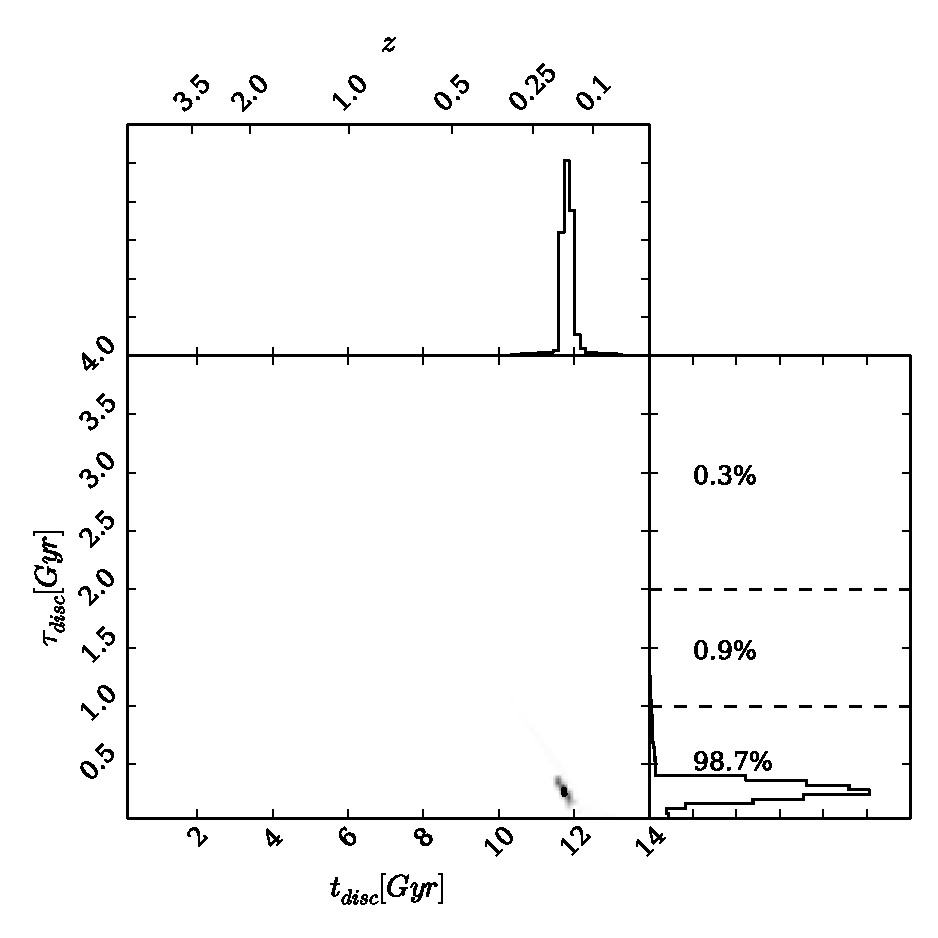
\includegraphics[width=0.55\textwidth]{morphology/blue_disc.pdf}}
\caption[Smooth and disc weighted opulation densities of blue cloud galaxies]{Contour plots showing the population densities for blue cloud galaxies in the \textsc{gz2-galex} sample, weighted by the morphological vote fractions from GZ2 to give both bulge (top) and disc (bottom) dominated distributions. The histograms show the projection into one dimension for each parameter. The dashed lines show the separation between rapid ($\tau ~\rm{[Gyr]} < 1.0$), intermediate ($1.0 < \tau ~\rm{[Gyr]} < 2.0$) and slow ($\tau ~\rm{[Gyr]} > 2.0$) quenching rates with the fraction of the combined posterior probability distribution in each region shown (see Section~\ref{stats}). Positions with probabilities less than 0.2 are discarded as poorly fit models, therefore unsurprisingly blue cloud galaxies are not well described by a quenching star formation model. }
\label{blue_c}
\end{figure*}

\begin{figure*}
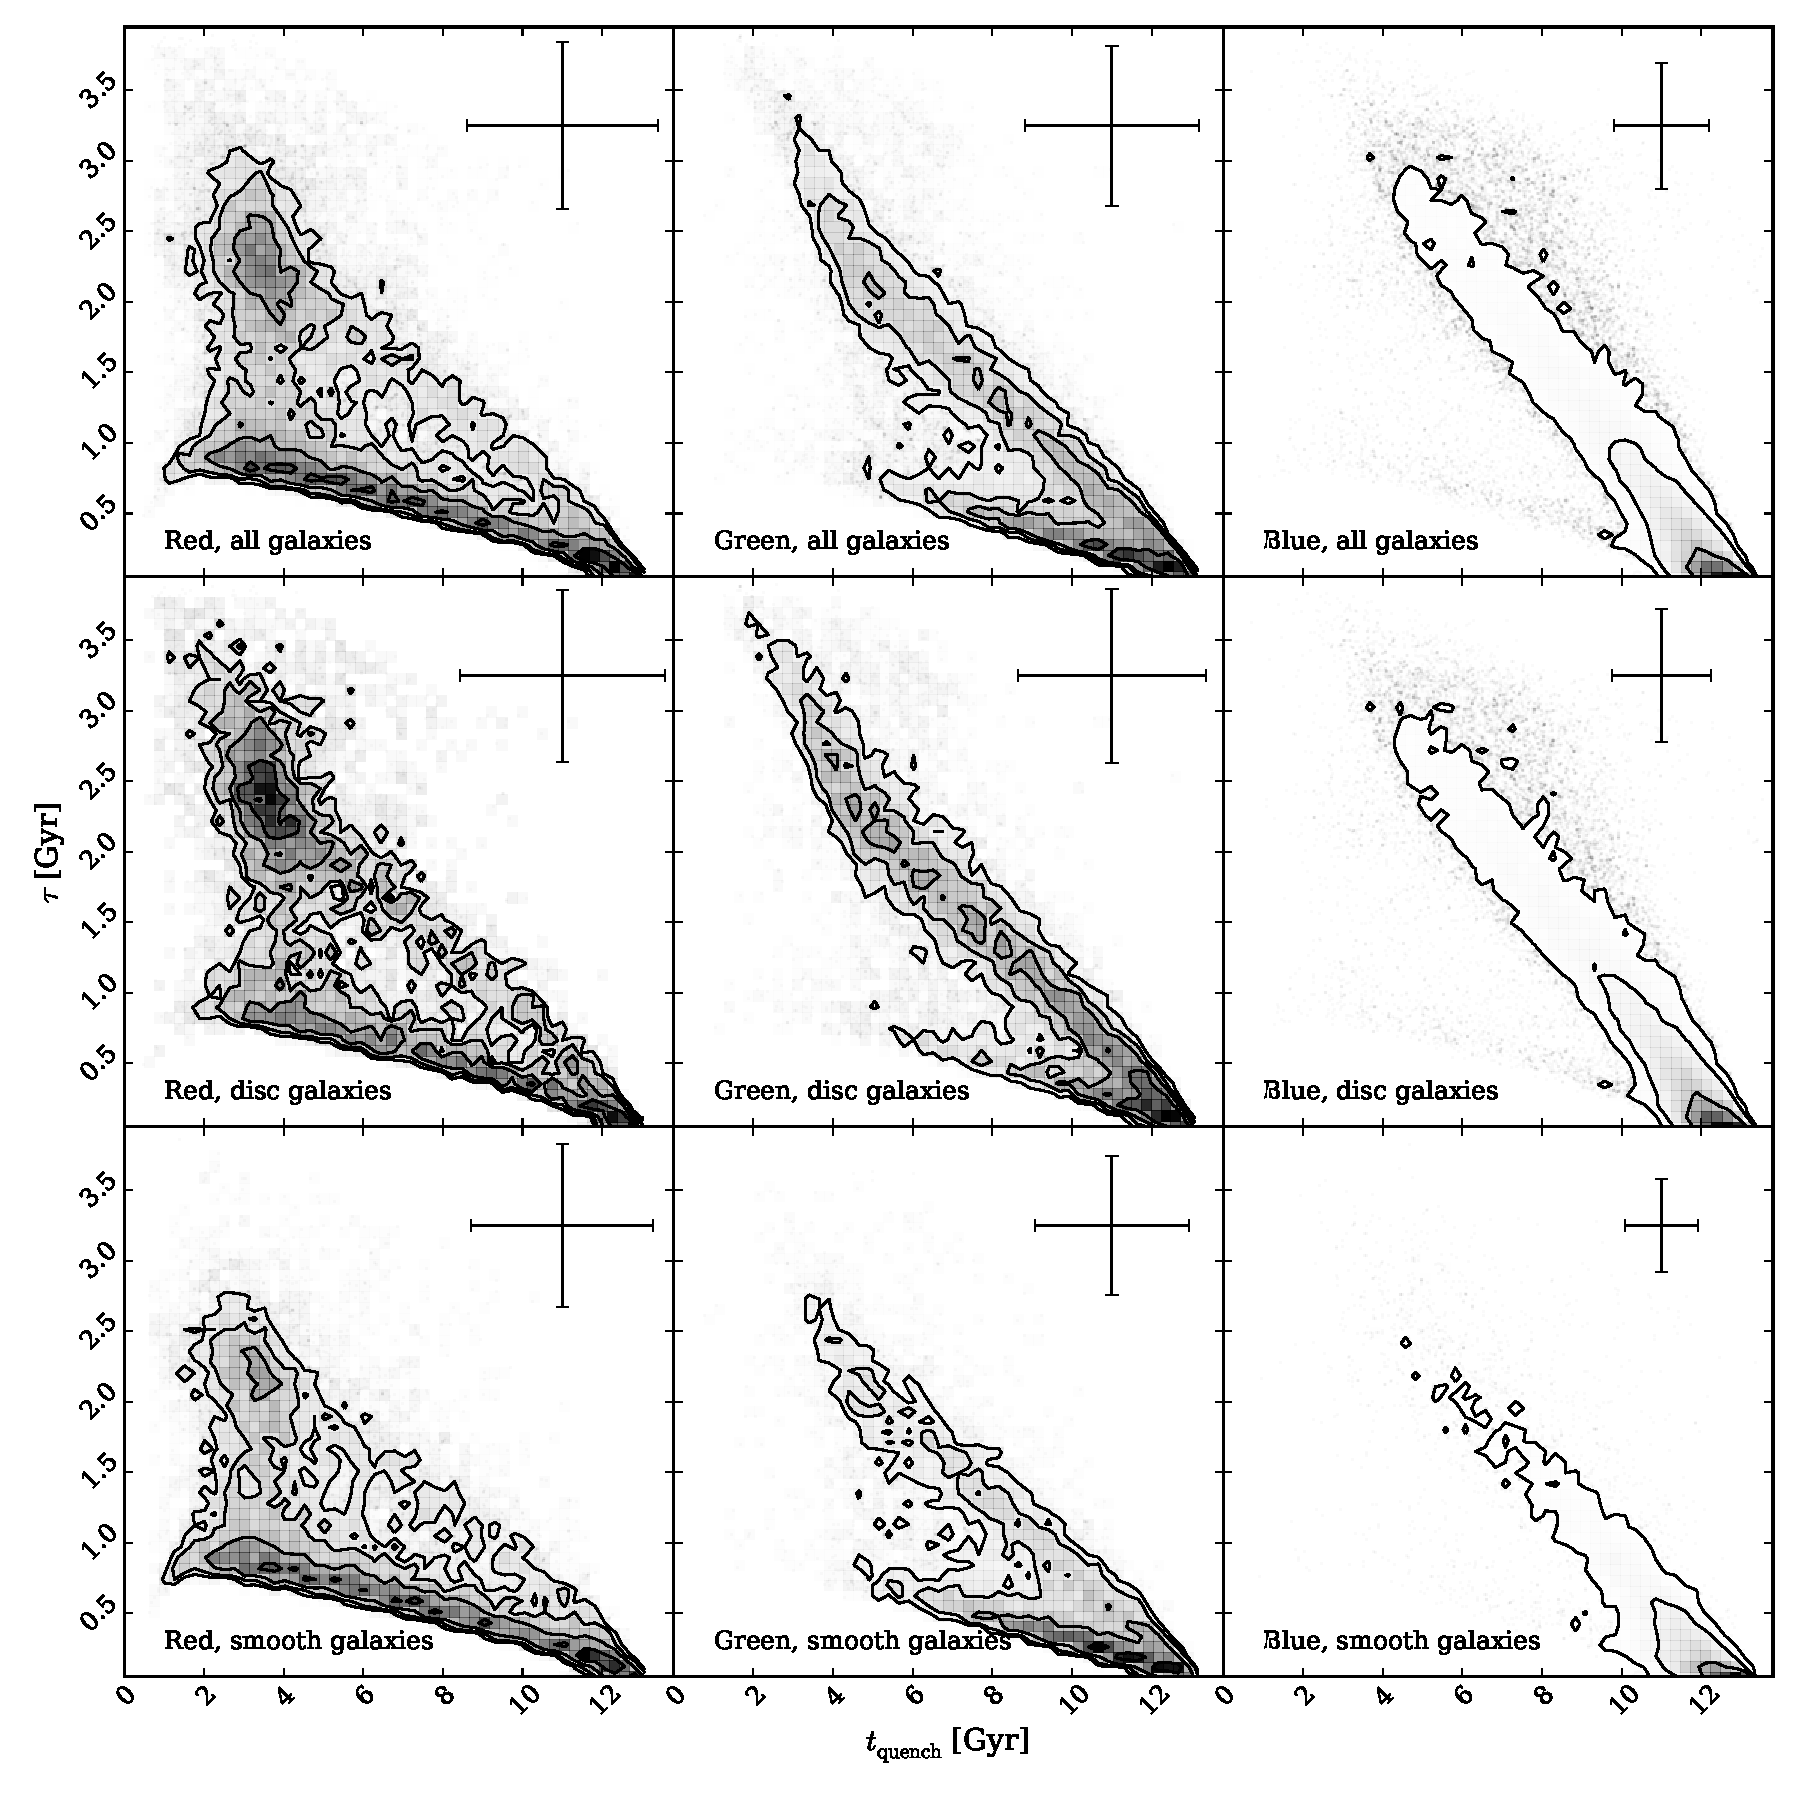
\includegraphics[width=0.95\textwidth]{morphology/contour_t_tau_mcmc_bestfit.pdf}
\caption[Best fit contours for red, green and blue clean galaxies]{Contours showing the positions in the $[t, \tau]$ parameter space of the median walker position (the 50th percentile; as shown by the intersection of the solid blue lines in Figure~\ref{one_example}) for each galaxy for all (top), disc ($p_d > 0.5$; middle), and smooth ($p_s > 0.5$; bottom) red sequence, green valley and blue cloud galaxies in the left, middle and bottom panels respectively. The error bars on each panel shows the average $68\%$ confidence on the median positions (calculated from the 16th and 84th percentile, as shown by the blue dashed lines in Figure~\ref{one_example}). These positions were calculated without discarding any walker positions due to low probability and without weighting by vote fractions, therefore this plot may be more intuitive than Figures~\ref{red_s},~\ref{green_v} \&~\ref{blue_c}. The differences between the smooth and disc populations and between the red, green and blue populations remain clearly apparent.}
\label{fig:bestfit}
\end{figure*}

Since the blue cloud by definition is made up of star forming galaxies, \starpy\ is expected to have some difficulty inferring any quenching model to describe them, as confirmed by Figure~\ref{blue_c}. The attempt to characterise a star forming galaxy with a quenched SFH model leads \starpy\ to attribute the extremely blue colours of the majority of these galaxies to a constant SFR until recent times and then a fast quench at the observed redshift (i.e. the colour has not had enough time to change from blue post-quench). 

This is particularly apparent for the blue disc weighted population. Perhaps even galaxies which are currently quenching slowly across the blue cloud cannot be well fit by the quenching models implemented, as they still have high SFRs despite some quenching. By definition although a galaxy is undergoing quenching, star formation can still be occurring, just at a slower rate than at earlier times. This rate is determined by $\tau$.

A very small fraction of the blue smooth weighted population density is found to begin quenching at redshifts $z \gtrsim 0.5 $ with slow quenching rates. These populations have been blue for a considerable period of time, slowly using up their gas for star formation by the Kennicutt$-$Schmidt law \citep{schmidt59, kennicutt97}. However the dominant fraction of the blue smooth weighted population density occurs at rapid quenching rates at recent times. This therefore provides some support to the theories for blue ellipticals as either merger-driven ($\sim76\%$; like those identified as recently quenched ellipticals with properties consistent with a merger origin by \citealt{McIntosh14}) or gas inflow-driven reinvigorated star formation that is now slowly decreasing ($\sim24\%$; such as the population of blue spheroidal galaxies studied by \citealt{Kaviraj13}).

The blue cloud is therefore primarily composed of both star forming galaxies of all morphologies and a smooth population undergoing a rapid quench, presumably after a previous event triggered star formation and turned them blue.


\section{Discussion}\label{morph:discussion}

In the previous section I presented the results of using \textsc{popstarpy} to derive the distribution of quenching histories for galaxies across the colour magnitude diagram. I  found differences between the SFHs of smooth- and disc-weighted populations of the red sequence, green valley and blue cloud. These results are summarised in Table~\ref{table:morphresults}. In this section I will speculate on the following question: what are the possible mechanisms driving these differences? 

\begin{table}[]
\centering
\caption{Table summarising the main results in Section~\ref{sec:morphresults} by describing the distributions derived for each population across the colour-magnitude diagram.}
\label{table:morphresults}
\resizebox{\textwidth}{!}{%
\begin{tabular}{rccc}
\hline
                                     & Red Sequence                                                                                 & Green Valley                                                                            & Blue Cloud                                                                       \\ \hline \hline
\multicolumn{1}{r|}{Smooth-weighted} & \begin{tabular}[c]{@{}c@{}}Dominated by \\ rapid \\ quenching rates\end{tabular}             & \begin{tabular}[c]{@{}c@{}}Dominated by \\ intermediate \\ quenching rates\end{tabular} & \begin{tabular}[c]{@{}c@{}}Dominated by \\ rapid \\ quenching rates\end{tabular} \\ \hline
\multicolumn{1}{r|}{Disc-weighted}   & \begin{tabular}[c]{@{}c@{}}Bimodal between \\ slow and rapid \\ quenching rates\end{tabular} & \begin{tabular}[c]{@{}c@{}}Dominated by \\ slow \\ quenching rates\end{tabular}         & -                                                                                \\ \hline
\end{tabular}%
}
\end{table}

\subsection{Rapid Quenching Rates}\label{rapid}

Rapid quenching is more dominant in the smooth weighted population densities than the disc weighted population (comparing top and bottom panels in Figures~\ref{red_s} \& \ref{green_v}). The red sequence populations also have larger fractions of rapid quenching rates than green valley population densities (compare Figures~\ref{red_s} \& \ref{green_v}).

This result suggests that rapid quenching mechanisms are accompanied by a change in morphology from a disc- to a smooth dominated galaxy as it quickly traverses the colour-magnitude diagram to the red sequence. This is supported by the number of disc galaxies that would need to undergo a morphological change in order for the smooth~:~disc ratio of galaxies in the green valley to match that of the red sequence (see Section~\ref{gv}). From this indirect evidence I suggest that this observed rapid quenching mechanism is major mergers. However, since a significant fraction of the red sequence disc weighted population density is found at rapid quenching rates (bottom panel Figure~\ref{red_s}), this suggests that the quenching may have occurred more rapidly than the morphological change in such a merger.

%Inspection of the individual galaxies dominating this area of the smooth weighted red population density reveals that this dominance of rapid quenching does not arise due to \emph{currently} merging galaxies. Although efforts were made to remove currently merging galaxies from the \textsc{gz2-galex} sample (using the GZ2 morphological vote fractions, see Section \ref{class}), this check was still performed to ensure no merging pairs were missed by the GZ users. Instead, the area is dominated by typical smooth galaxies with both red optical and NUV colours. Although a prescription for modelling a merger in the SFH is not included in this work the after-effects can still be detected (see Section \ref{future} for future work planned with \starpy).

In order to achieve such rapid quenching rates ($\tau \lesssim 0.5$) in a simulation of a major merger, \citet*{springel05b} showed that feedback from black hole activity is necessary. As discussed in Chapter~\ref{chap:intro}, powerful quasar outflows are thought to be able to remove much of the gas from the inner regions of the galaxy, terminating star formation on extremely short rates (this connection between quenching and AGN feedback is explored further in Chapter~\ref{chap:agn}). \citet{bell06}, using data from the COMBO-17 redshift survey ($0.4 < z < 0.8$), estimate a merger timescale of $\sim 0.4~\rm{Gyr}$ for the merger to go from being classified as a close galaxy pair to morphologically disturbed. \citet*{springel05b} consequently find using hydrodynamical simulations that after $\sim1~\rm{Gyr}$ the merger remnant has reddened to $u-r \sim 2.0$. 

Under the simple assumption that the merger timescale will be $\sim$ quenching rate, these simulation results are in agreement with the simple exponential quenching models used here. Figure~\ref{sfr_mass_col} shows that SFH models with $\tau < 0.4~\rm{Gyr}$ have reached $u-r ~\gtrsim 2.2$, within $\sim1~\rm{Gyr}$. This could explain the fraction of the red disc weighted population with very rapid quenching rates. These galaxies may have undergone a major merger recently but are still undergoing a morphological change from disc, to disturbed, to an eventual smooth galaxy (see also \citealt{vdW09}). Similarly they may have retained their disc structure in a merger, such as in recent simulations by \citet{pontzen16}. This possible connection between AGN feedback and rapid quenching rates is explored further in Chapter~\ref{chap:agn}. 

These rapid quenching rates, while found across all populations, do not fully characterise the entire red sequence or green valley populations. Dry (i.e. gas poor) major mergers therefore cannot fully account for the formation of any galaxy population, supporting the observational conclusions of \citet{Bell07,Bundy07, kaviraj14a} and simulations by \citet{Genel08}. 

\subsection{Intermediate Quenching Rates}\label{int}

Intermediate quenching rates are found to be equally prevalent across both smooth and disc weighted populations across cosmic time and are particularly dominant in the green valley (see Figure~\ref{green_v}). This suggests that this intermediate quenching rate must therefore be caused by mechanisms that both preserve and transform morphology. It is this result of another route through the green valley that is in contradiction with the findings of S14. 

I propose that these intermediate quenching rates ($1 \leq \tau~\rm{[Gyr]} \leq 2$) are caused by any of the following: gas rich major mergers, major mergers without black hole feedback, minor mergers and galaxy interactions. This is supported by the findings of \citet{Lotz11}, who find in simulations that increasing the baryonic gas fraction in a merger (mass ratios $\sim 1:1-1:4$) causes the observability timescale of the merger to increase from $\sim0.2~\rm{Gyr}$ (with little gas, as above for major mergers which can cause rapid quenching rates) up to $\sim1.5~\rm{Gyr}$ (with large gas fractions). 

Intermediate quenching rates are equally dominant for both smooth and disc populations across Figures~\ref{red_s} and~\ref{green_v}. \citet{lotz08b} show that the remnants of simulated equal mass gas rich disc mergers are observable for $\gtrsim1~\rm{Gyr}$ post merger and state that they appear ``disc-like and dusty" in the simulations, which is consistent with an ``early-type spiral morphology".  Such galaxies are often observed to have spiral features with a dominant bulge, suggesting that such galaxies may divide the votes of the GZ2 users, producing vote fractions of $p_s \sim p_d \sim 0.5$. Such a vote fraction may also arise because the galaxy is at a large distance or because it is an S0 galaxy whose morphology can be interpreted by different GZ2 users in different ways. \citet{GZ2} find that S0 galaxies expertly classified by \citet{nair10} are more commonly classified as ellipticals by GZ2 users, but that the population has a significant tail to high disc vote fractions. A galaxy with these ambiguous GZ2 vote fractions will therefore contribute equally to the smooth and disc weighted population densities which may explain the dominance of these intermediate quenching rates across all populations. 

By inspecting Figure~\ref{pred}, we find that SFH models with these intermediate quenching rates of $1.0 \lesssim ~\tau~\rm{[Gyr]} ~\lesssim 2.0$ take approximately $2.5-5.5~\rm{Gyr}$ to reach the red sequence. In the simulations of \citet*{springel05b} which do not include feedback from black holes, merger remnants can sustain low levels of star formation for several Gyrs if a small fraction of gas is not consumed in the merger triggered starburst (either because the mass ratio is not large enough or from the lack of strong black hole activity). The remnants from these simulations take $\sim5.5~\rm{Gyr}$ to reach red optical colours of $u-r \sim 2.1$, providing support for the hypothesis that the intermediate quenching rates may be caused by minor mergers. 

Observationally, \citet{Darg10a} showed an increase in the spiral to elliptical ratio for merging galaxies ($0.005 < z < 0.1$) by a factor of two compared to the typical galaxy population. They attribute this to the mergers of spirals being observable for much longer compared to mergers with elliptical galaxies. This supports the hypothesis that the slower quenching rates in the $\tau < 1.5 ~\rm{Gyr}$ region of the disc weighted green valley population density (see bottom panel of Figure~\ref{green_v}) may be caused by a minor or wet major merger and eventually give rise to the morphological change needed to match the ratio of smooth:disc galaxies seen in the red sequence (see Section \ref{gv}). 
 
 \citet{Darg10a} also show (in their Figure 6) that below a merger ratio of $1:10$ (up to $\sim 1:100$), green is the dominant average galaxy colour of visually identified merging pairs in GZ. These pairs are also dominated by spiral-spiral mergers as opposed to elliptical-elliptical and elliptical-spiral mergers. The remnants of these green spiral-spiral mergers would contribute to the green disc weighted population density in the bottom panel of Figure~\ref{green_v}, where these intermediate quenching rates are found to be the dominant SFH. This lends more support to the idea that these intermediate quenching rates are caused in part by minor mergers. 

For the smooth weighted green valley population (shown in the top panel of Figure~\ref{green_v}), $40.6\%$ of the distribution is found in the intermediate quenching rate regime. Similarly, \citet{kaviraj14a, kaviraj14b} by studying SDSS photometry ($z<0.07$) state that approximately half of the star formation in all galaxies is driven by minor mergers at $0.5 < z < 0.7$. These minor mergers would therefore exhaust available gas for star formation and consequently causing a gradual decline in the star formation rate. This is therefore complimentary to the fraction of smooth green valley galaxies found to be undergoing quenching at an intermediate rate in the top panel of Figure~\ref{green_v}.

Assuming that rapid and intermediate quenching rates are therefore caused by major or minor mergers, the fraction of population density with $\tau \leq 2~\rm{Gyr}$ can provide an estimate for the percentage of galaxies with a merger dominated evolutionary history.  This is calculated to be $73.9\%$ and $59.3\%$, for the smooth weighted red sequence and green valley populations (top panels Figures~\ref{red_s} and~\ref{green_v}) respectively. This estimate for the faction of smooth galaxies with merger dominated histories is supported by the earlier work of \cite{kaviraj11}. They use multi wavelength photometry of galaxies in COSMOS \citep{Scoville07} to estimate that $70\%$ of early-type galaxies appear morphologically disturbed, suggesting either a minor or major merger in their history. Note that the star formation model used here is a basic one and has no prescription for reignition of star formation post-quench. Such a reignition of star formation has been detected observationally by \cite{kaviraj11} and seen in simulations by \cite{pontzen16}.

Any external event which can cause either a burst of star formation (depleting the gas available) or directly strip a galaxy of its gas, for example galaxy harassment, interactions, ram pressure stripping, strangulation and interactions internal to clusters, should also cause quenching with an intermediate rate. Such mechanisms would be the dominant cause of quenching in dense environments; considering that the majority of galaxies reside in groups or clusters (\citealt{Coil08} find that green valley galaxies are just as clustered as red sequence galaxies). It is not surprising therefore that the majority of the \textsc{gz2-galex} galaxies ($\sim50\%$) are classified with intermediate morphology (i.e., $p_d \sim p_s \sim 0.5$, see Table~\ref{table:subs}) and therefore may be undergoing or have undergone such an interaction. This obvious dependency of the quenching parameters on the galaxy environment will be investigated further in Chapter~\ref{chap:env}.


\subsection{Slow Quenching Rates}\label{slow}

Although intermediate and rapid quenching rates are the dominant mechanisms across the colour-magnitude diagram, together they cannot completely account for the quenching of disc galaxies. S14 concluded that slow quenching rates were the most dominant mechanism for disc galaxies. However I show that: (i) intermediate quenching rates are equally important in the green valley (bottom panel Figure \ref{green_v}) and (ii) rapid quenching rates are equally important in the red sequence (bottom panel Figure ~\ref{red_s}). There is also a significantly lower fraction of slow quenching rates in the smooth weighted population densities (top panels of Figures~\ref{red_s} \& \ref{green_v}). This suggests that the evolution (or indeed creation) of typical smooth galaxies is dominated by processes external to the galaxy. The exceptions are galaxies in the blue cloud where a small fraction of the smooth weighted population density is found at slow quenching rates (top panel Figure~\ref{blue_c}), which could be due to a reinvigoration of star formation that is slowly depleting the available gas (via the Kennicutt$-$Schmidt law).

Table~\ref{table:subs} shows that $3.9\%$ of the \textsc{gz2-galex} sample are red sequence late-type galaxies, i.e. red late-type spirals. This is, within uncertainties, in agreement with the findings of \citet{masters10c}, who find $\sim6\%$ of late-type spirals are red when defined by a cut in the $g-r$ optical colour (rather than with $u-r$ as used in this investigation) and are at the `blue end of the red sequence'. \citet{Bamford09}, using GZ1 vote fractions of galaxies in the SDSS, found a significant fraction of field galaxies are in fact high stellar mass red spiral galaxies. As these galaxies are isolated from the effects of interactions from other galaxies, the slow quenching mechanisms dominant in the disc weighted population densities (bottom panels of Figures~\ref{red_s} \& \ref{green_v}) are most likely due to secular processes (i.e. mechanisms internal to the galaxy, in the absence of sudden accretion or merger events; \citealt{kormendy04, Sheth12}). Bar formation in a disc galaxy is such a mechanism, whereby gas is funnelled to the centre of the galaxy by the bar over long rates where it is used for star formation \citep{masters12a, saintonge12, Cheung13}, consequently forming a `pseudo-bulge' \citep{Kormendy10, Simmons13}.

I therefore speculate that these slow quenching rates are due to secular evolution, as such processes do not change the disc dominated nature of a galaxy. 

\section{Conclusions}\label{morph:conc}

I have used morphological classifications from the Galaxy Zoo 2 project to determine the morphology-dependent star formation histories of galaxies via a Bayesian analysis of an exponentially declining star formation quenching model. The most likely values were determined for the quenching onset time, $t_q$, and quenching timescale, $\tau$, in this model for galaxies across the blue cloud, green valley and red sequence to trace the morphological dependence of galactic evolution across the colour-magnitude diagram. 

The green valley is found to be a transitional population for all morphological types (in conflict with S14), however this transition proceeds slowly for a significant fraction of disc dominated galaxies and occurs rapidly for the majority of smooth dominated galaxies in the red sequence (in agreement with S14). However, in addition to the results of S14, the inclusion of both (i) the entire \textsc{gz2-galex} sample with no morphology thresholds, and (ii) a robust statistical analysis of the results has revealed a more nuanced result; specifically that the prevailing mechanism across all morphologies and populations is quenching with intermediate rates. The main findings are summarised as follows:
\begin{enumerate}[(i)]
\item Quenching within the red sequence population occurs at earlier quenching times (i.e. higher redshift) than in the green valley population regardless of morphology (see Figures~\ref{red_s} and~\ref{green_v}). Therefore the quenching mechanisms currently occurring in the green valley were also active in creating the `blue end of of the red sequence' at earlier times; confirming that the green valley is indeed a transitional population, regardless of morphology.

\item The red sequence is dominated by galaxies which are elliptical in morphology and have undergone a rapid to intermediate quench at some point in cosmic time, resulting in a very low current SFR (see Section~\ref{rs}).

\item The green valley as it is currently observed is dominated by very slowly evolving disc dominated galaxies along with intermediate and smooth dominated galaxies which pass across it with intermediate rates within $\sim 1.0-1.5~\rm{Gyr}$ (see Section~\ref{gv}).

\item There are many different mechanisms responsible for quenching, all causing a galaxy to progress through the green valley. These mechanisms are dependent on galaxy type, with the smooth and disc dominated galaxies each having different dominant star formation histories across the colour-magnitude diagram. 

\item Blue cloud galaxies are not well fit by a quenching model of star formation due to the continuous high star formation rates occurring (see Figure~\ref{blue_c}).

\item Rapid quenching rates are found at a lower fraction in the green valley population than the red sequence population (see Figures~\ref{red_s} \& \ref{green_v}). I speculate that this quenching mechanism is caused by major mergers with black hole feedback, which are able to expel the remaining gas not initially exhausted in the merger-induced starburst and which can cause a change in morphology from disc- to bulge-dominated. The colour-change rates from previous simulations of such events agree with the derived quenching rates (see Section~\ref{rapid}). These rapid quenching rates are instrumental in forming red galaxies, however galaxies at the current epoch passing through the green valley do so at more intermediate quenching rates (see Figure~\ref{green_v}).

\item Intermediate quenching rates ($1.0 < ~\tau~\rm{[Gyr]}~ < 2.0 $) are found with constant density across red and green galaxies for both smooth- and disc-weighted populations, the rates for which agree with observed and simulated minor merger rates (see Section~\ref{int}). I hypothesise that such rates can also be caused by a number of external processes, including gas rich major mergers, mergers without black hole feedback, galaxy harassment, interactions, strangulation and ram pressure stripping. The rates and observed morphologies from previous studies agree with the results, including that this is the dominant mechanism for intermediately classified galaxies such as early-type spiral galaxies with spiral features but a dominant bulge, which split the GZ2 vote fractions (see Section~\ref{int}). 

\item Slow quenching rates are the most dominant mechanism in the disc galaxy population across the colour-magnitude diagram population (see bottom panels Figures~\ref{red_s} \& \ref{green_v}). Disc galaxies are often found in the field, therefore I hypothesise that such slow quenching rates are caused by secular evolution and processes internal to the galaxy (see Section \ref{bc}). A small amount of slow quenching rates is also detected for blue elliptical galaxies which is attributed to a reinvigoration of star formation, the peak of which has passed and has started to decline by slowly depleting the gas available (see Section~\ref{bc}). 
\end{enumerate}
